\chapter{Ejemplos completos}
\section{Simplificacion de fronteras basada en cubrimiento}\label{EXE:sfbc}
\begin{figure}[H]
  \centerfloat
  \subfloat[Estado inicial.]{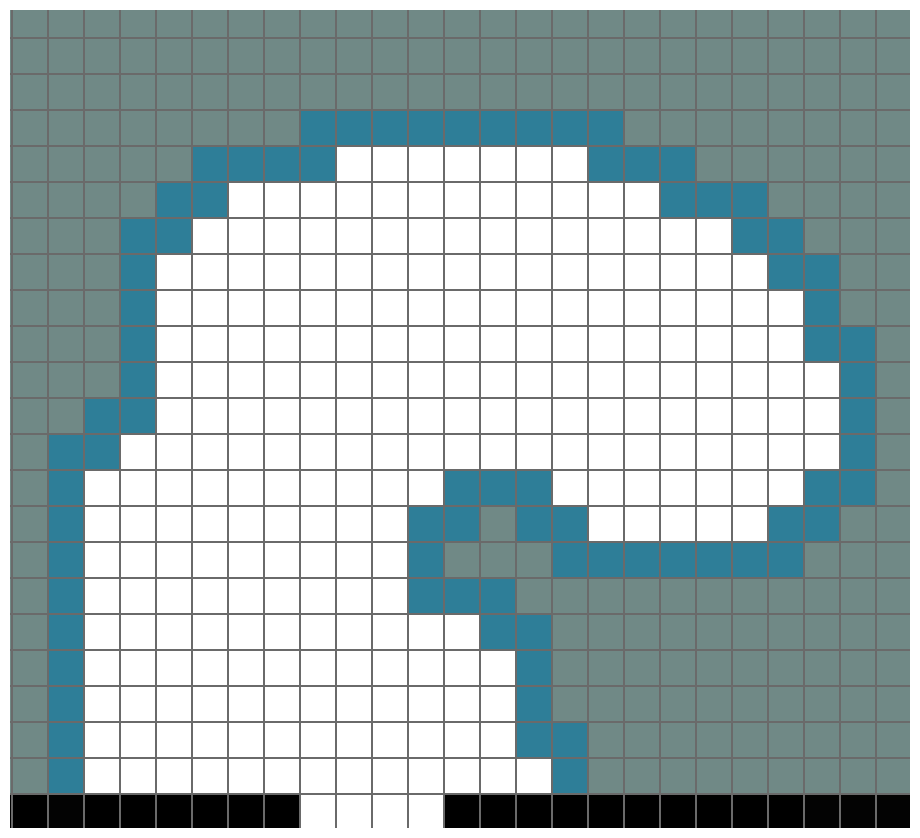
\includegraphics[clip=true, width=0.40\textwidth]{imagenes/ejemploSimpCub/a1.png}}
  \subfloat[Se inicializa $\mli{FP}$.]{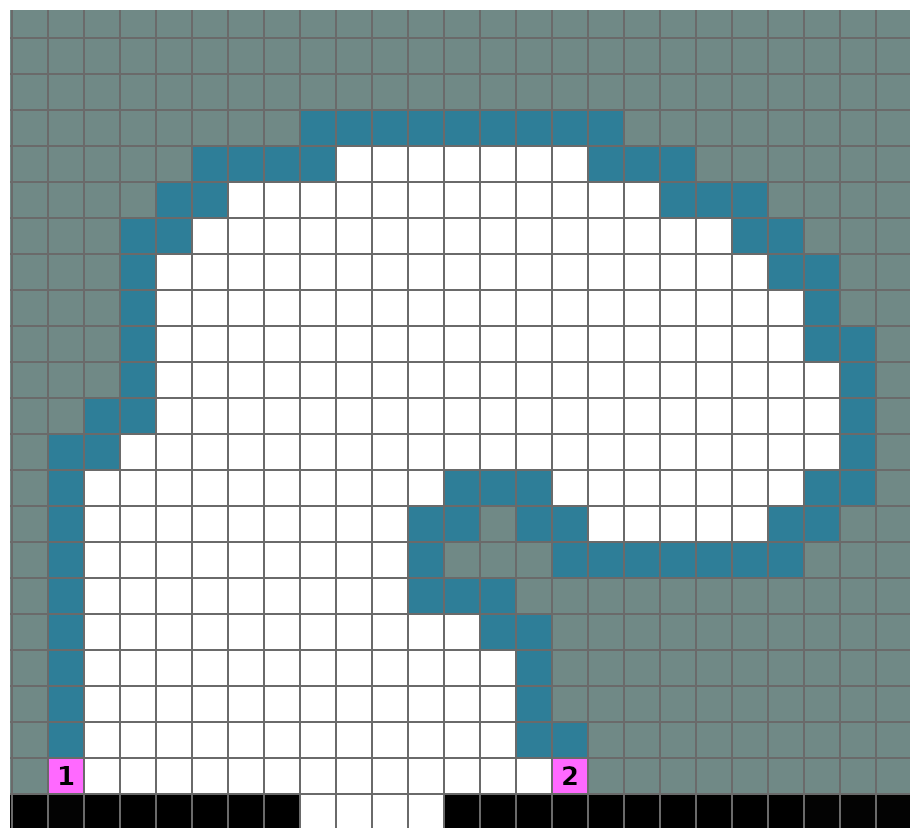
\includegraphics[clip=true, width=0.40\textwidth]{imagenes/ejemploSimpCub/a2.png}}

  \subfloat[Se obtiene $\mli{fp}$ desencolando de $\mli{FP}$.]{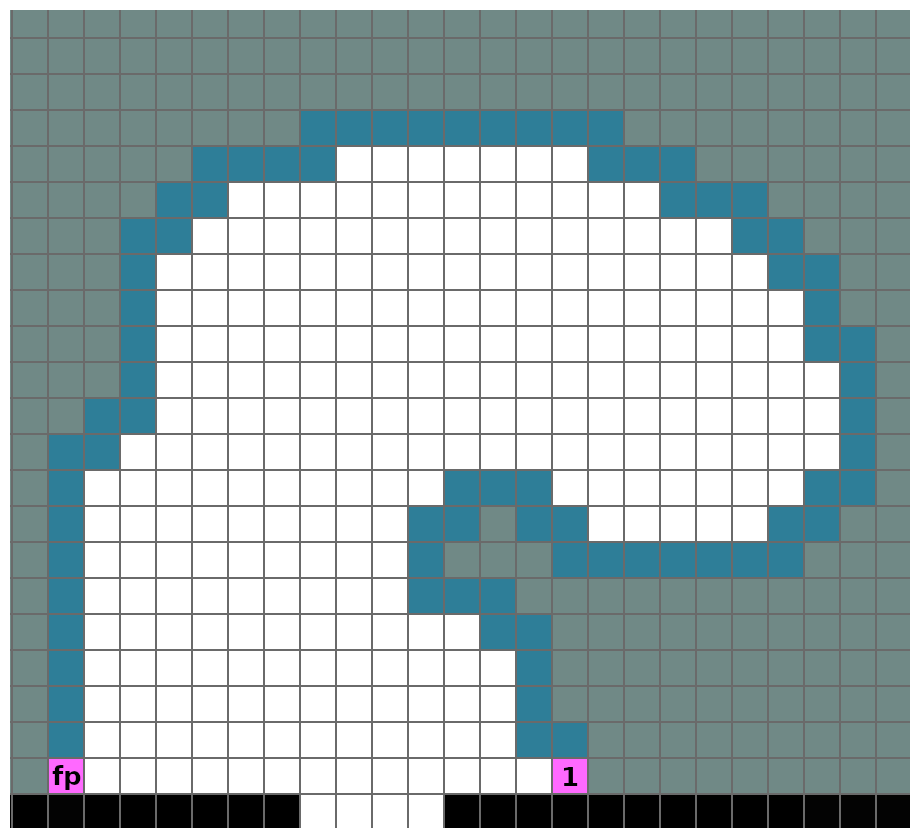
\includegraphics[clip=true, width=0.40\textwidth]{imagenes/ejemploSimpCub/b1.png}}
  \subfloat[Existen celdas mas alejadas que $2*rango$, los candidatos se obienen con $radio=rango$. ]{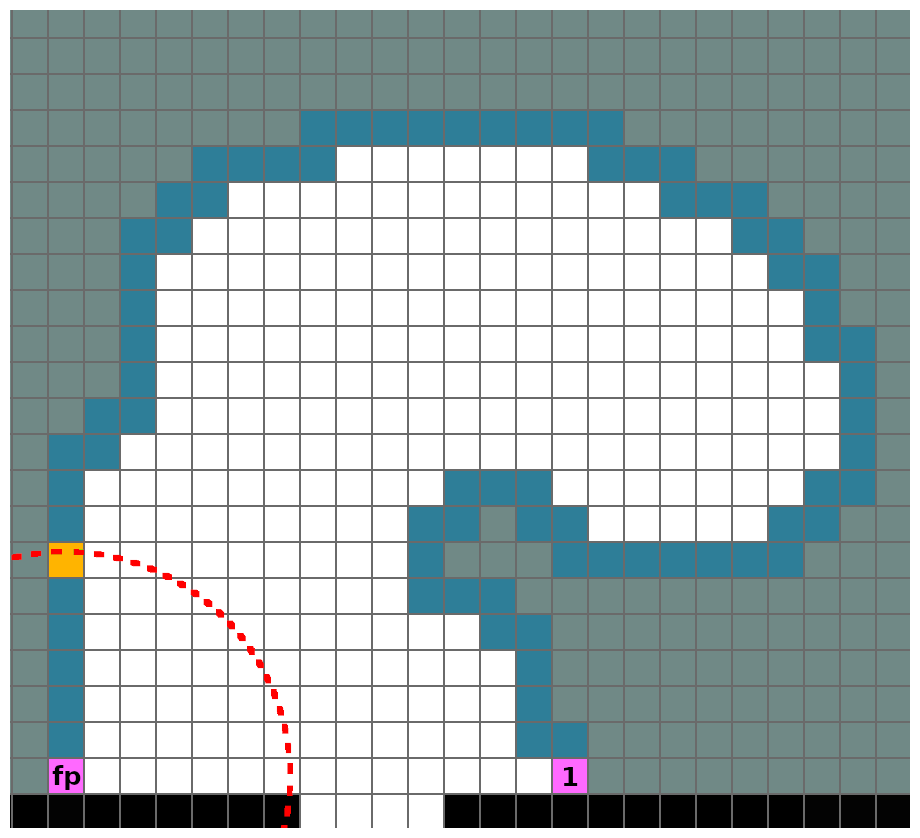
\includegraphics[clip=true, width=0.40\textwidth]{imagenes/ejemploSimpCub/b3.png}}
  \subfloat[Se elige el unico candidato como $\mli{fs}$, se actualiza $\mli{UF}$, $\mli{FS_i}$ y $\mli{FP}$.]{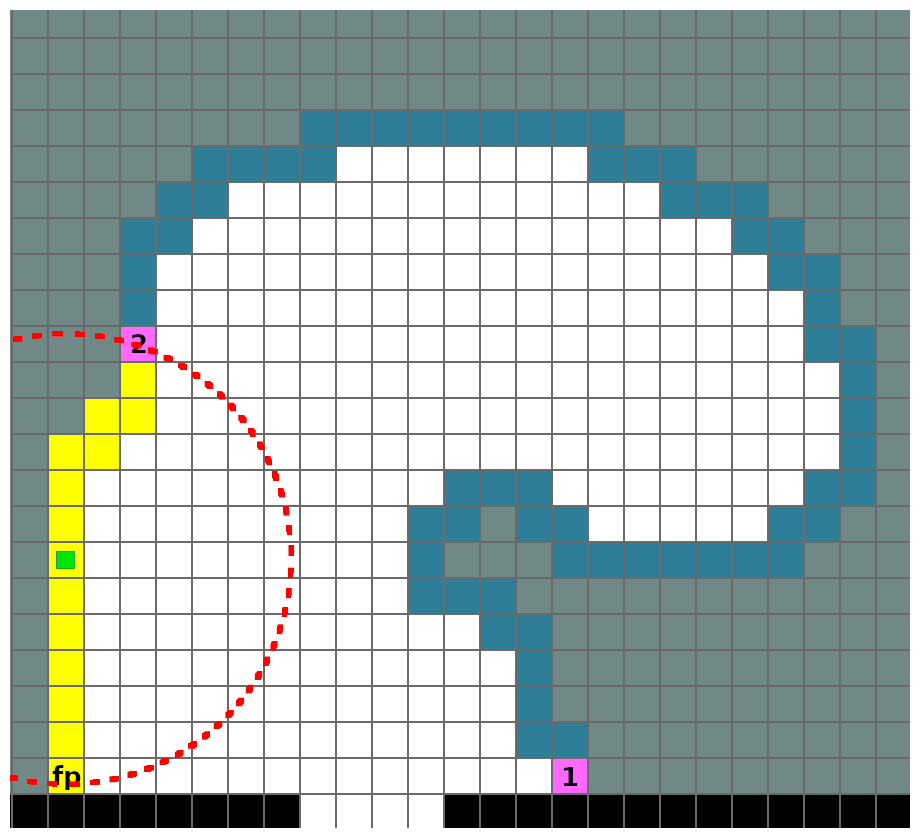
\includegraphics[clip=true, width=0.40\textwidth]{imagenes/ejemploSimpCub/b5.png}}
 \phantomcaption

\end{figure}

\begin{figure}[H]
  \setcounter{subfigure}{5}
  \centerfloat
  \subfloat[Se obtiene $\mli{fp}$ desencolando de $\mli{FP}$.]{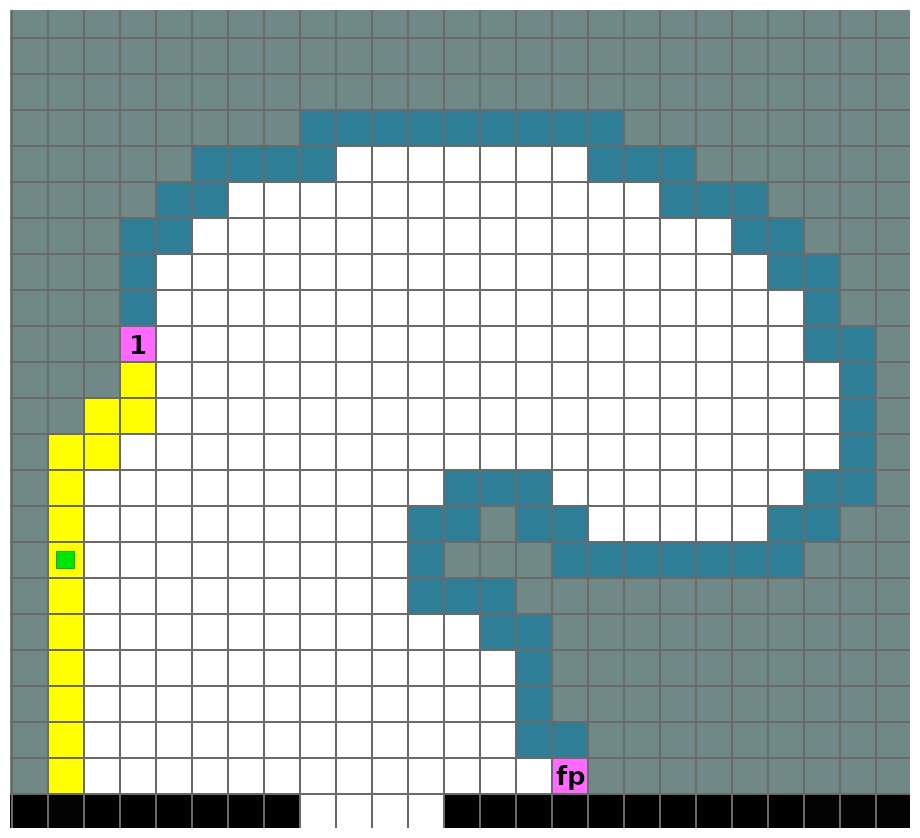
\includegraphics[clip=true, width=0.40\textwidth]{imagenes/ejemploSimpCub/c1.png}}
  \subfloat[Existen celdas mas alejadas que $rango$, los candidatos se obienen con $radio=rango$. ]{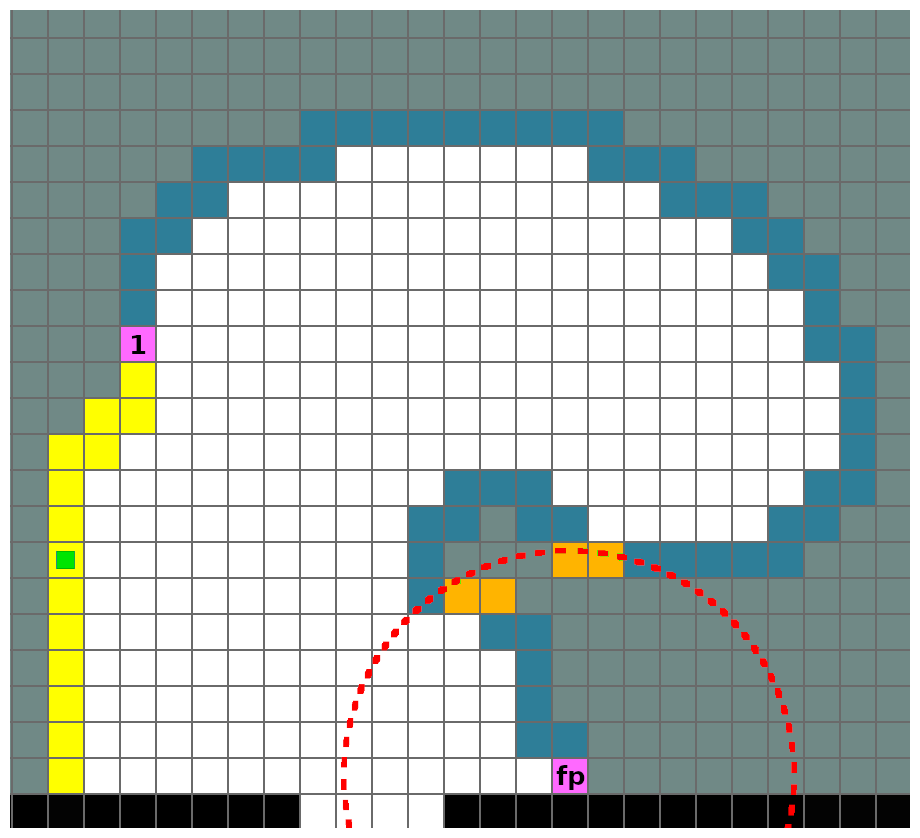
\includegraphics[clip=true, width=0.40\textwidth]{imagenes/ejemploSimpCub/c3.png}}
  \subfloat[Se elige arbitrariamente un candidato como $\mli{fs}$, se actualiza $\mli{UF}$, $\mli{FS_i}$ y $\mli{FP}$.]{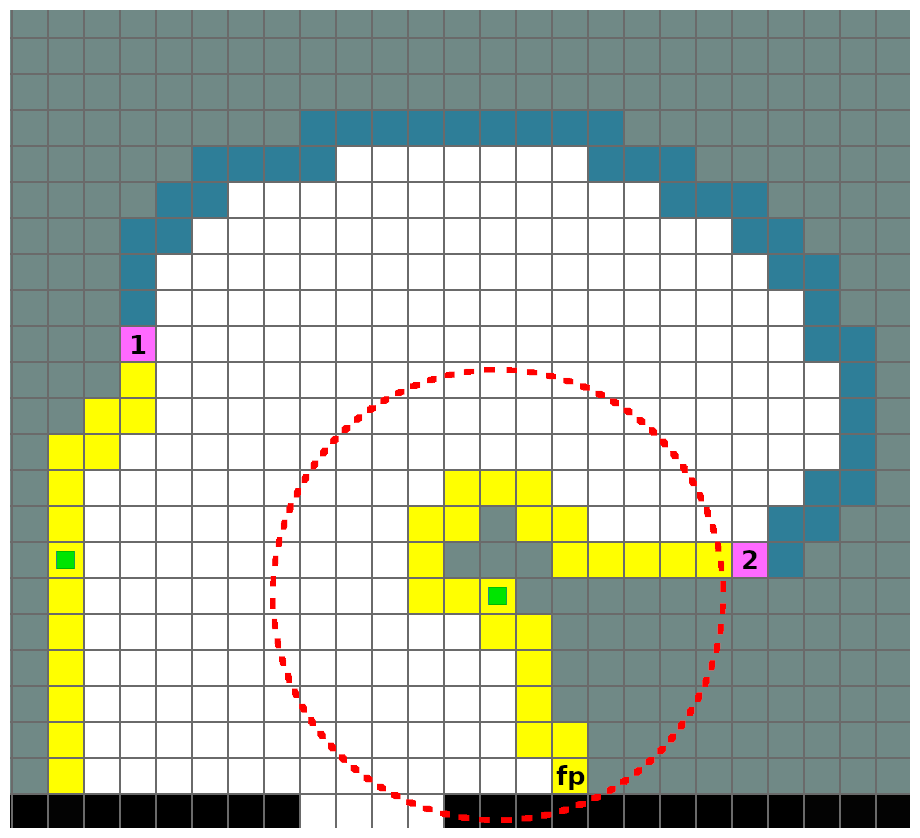
\includegraphics[clip=true, width=0.40\textwidth]{imagenes/ejemploSimpCub/c5.png}}


  \subfloat[Se obtiene $\mli{fp}$ desencolando de $\mli{FP}$.]{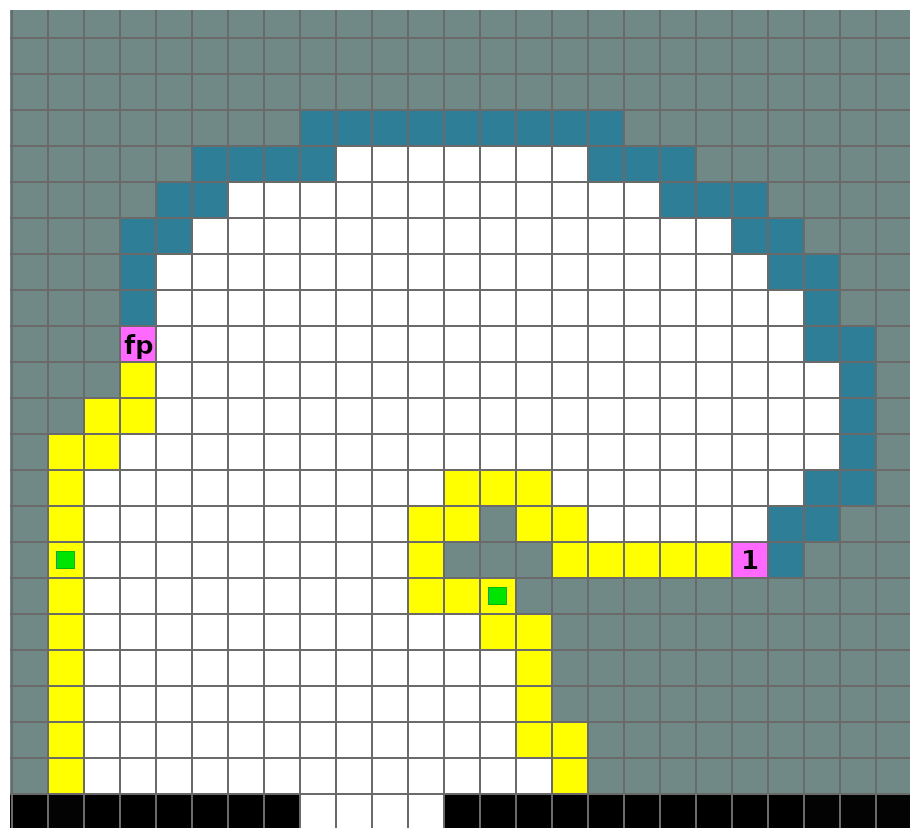
\includegraphics[clip=true, width=0.40\textwidth]{imagenes/ejemploSimpCub/d1.png}}
  \subfloat[Existen celdas mas alejadas que $2*rango$, los candidatos se obienen con $radio=rango$. ]{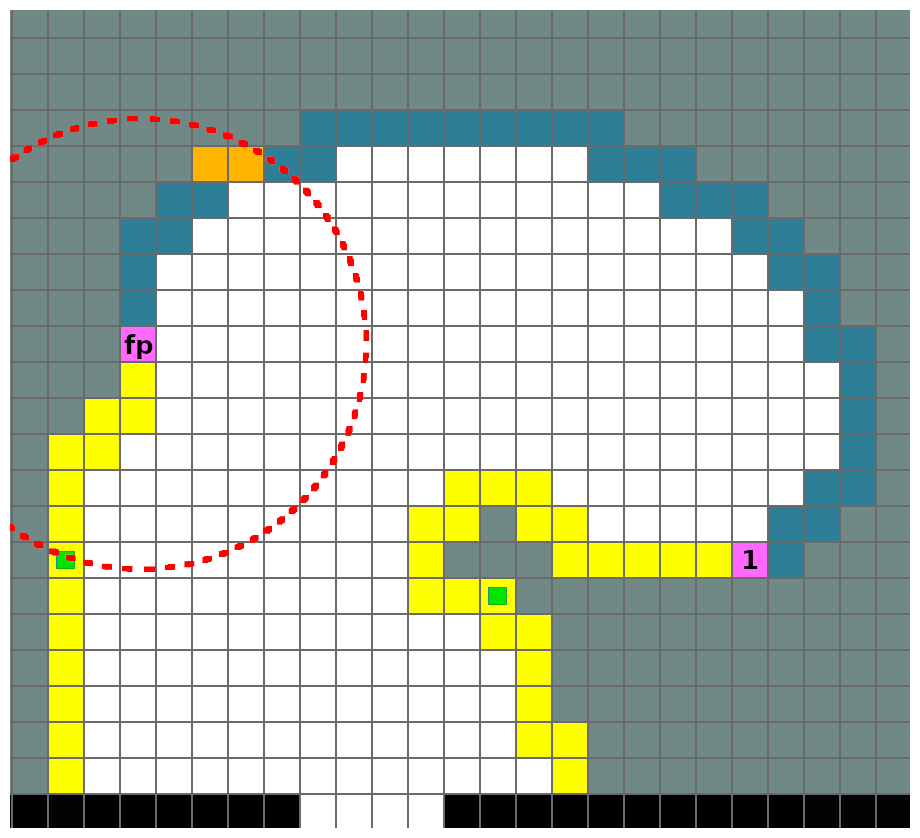
\includegraphics[clip=true, width=0.40\textwidth]{imagenes/ejemploSimpCub/d3.png}}
  \subfloat[Se elige arbitrariamente un candidato como $\mli{fs}$, se actualiza $\mli{UF}$, $\mli{FS_i}$ y $\mli{FP}$.]{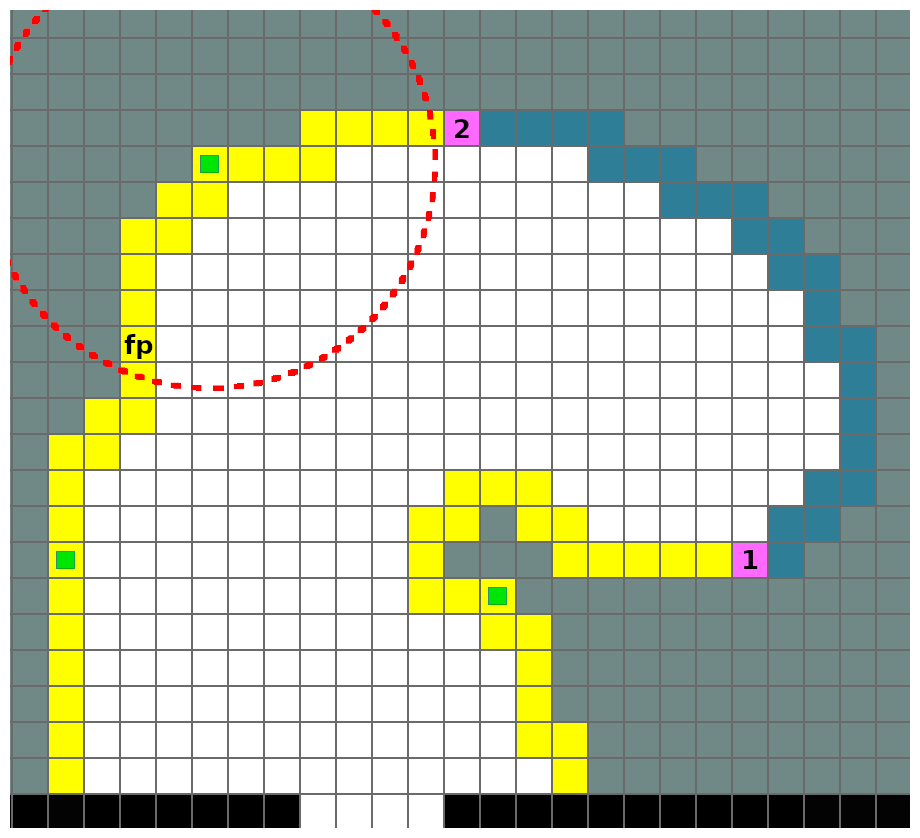
\includegraphics[clip=true, width=0.40\textwidth]{imagenes/ejemploSimpCub/d5.png}}

  \subfloat[Se obtiene $\mli{fp}$ desencolando de $\mli{FP}$.]{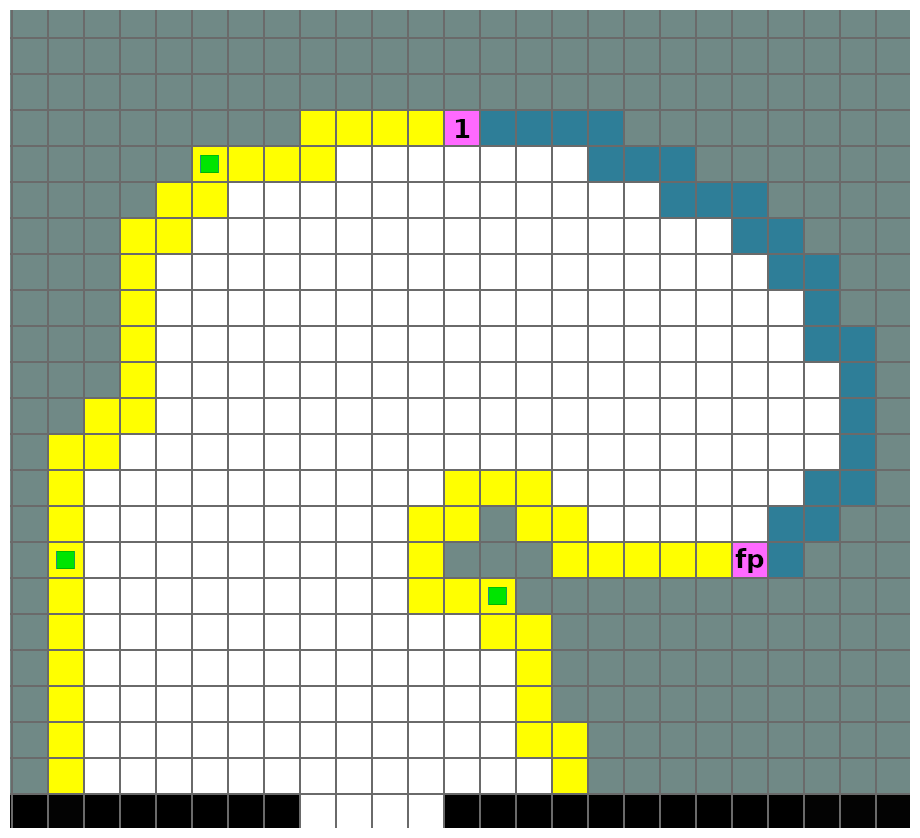
\includegraphics[clip=true, width=0.40\textwidth]{imagenes/ejemploSimpCub/e1.png}}
  \subfloat[Existen celdas mas alejadas que $2*rango$, los candidatos se obienen con $radio=rango$. ]{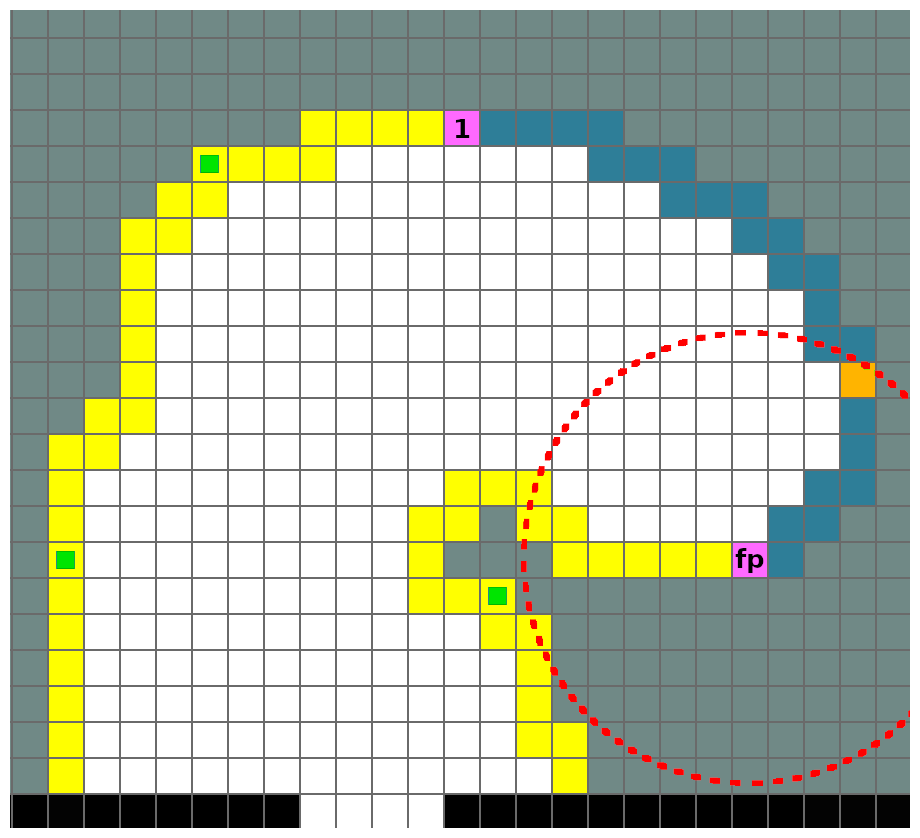
\includegraphics[clip=true, width=0.40\textwidth]{imagenes/ejemploSimpCub/e3.png}}
  \subfloat[Se elige arbitrariamente un candidato como $\mli{fs}$, se actualiza $\mli{UF}$, $\mli{FS_i}$ y $\mli{FP}$.]{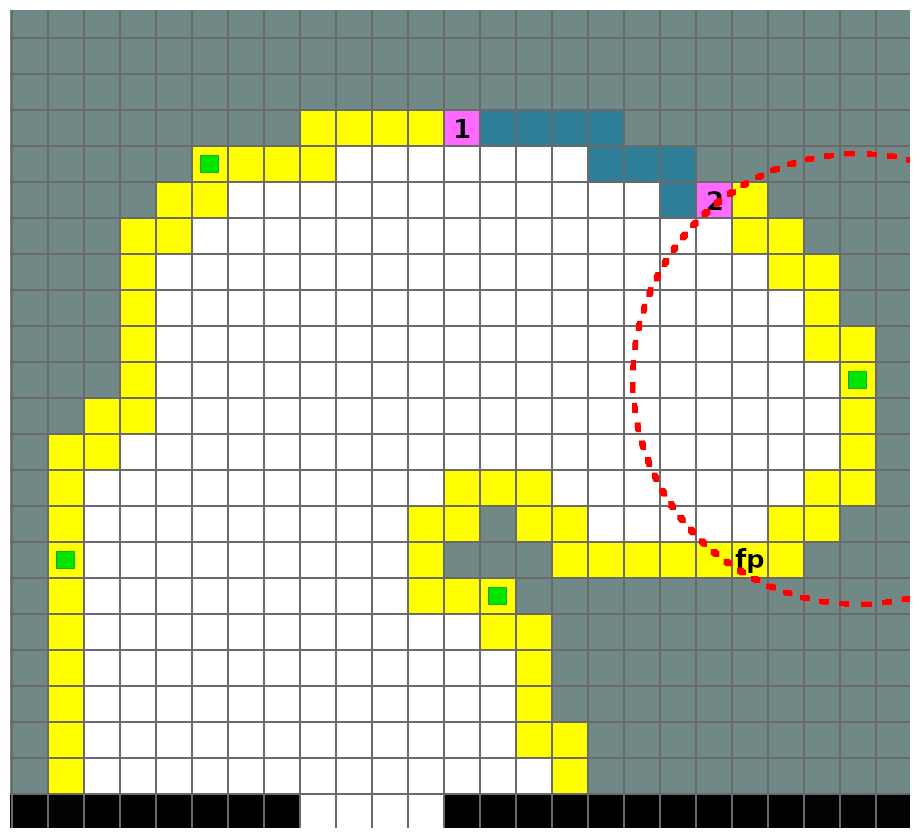
\includegraphics[clip=true, width=0.40\textwidth]{imagenes/ejemploSimpCub/e5.png}}

 \phantomcaption
\end{figure}

\setcounter{figure}{0}

\begin{figure}[H]
  \setcounter{subfigure}{14}
  \centerfloat

  \subfloat[Se obtiene $\mli{fp}$ desencolando de $\mli{FP}$.]{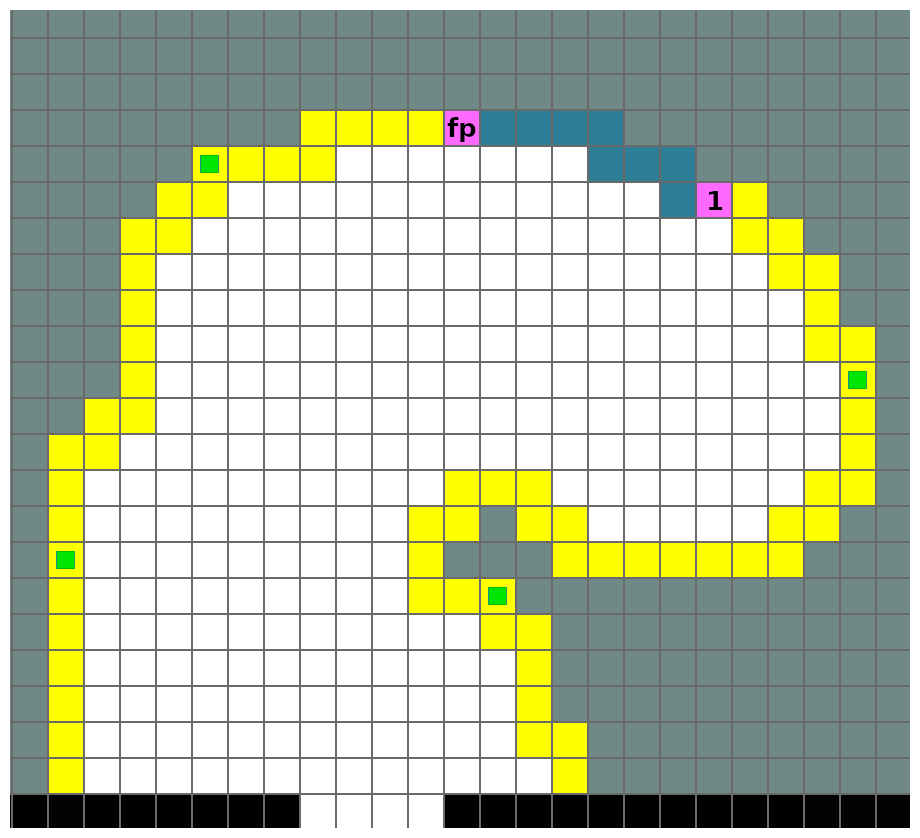
\includegraphics[clip=true, width=0.40\textwidth]{imagenes/ejemploSimpCub/f1.png}}
  \subfloat[No existen celdas mas alejadas que $2*rango$, los candidatos se obienen con $radio=3.45$ (largos de celda). ]{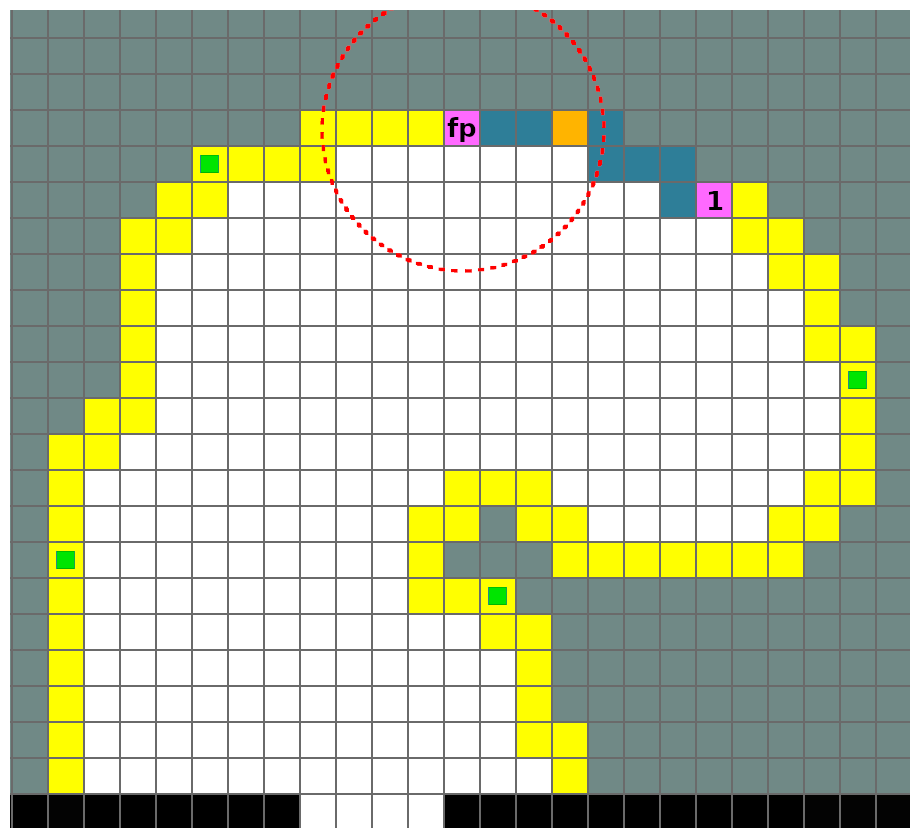
\includegraphics[clip=true, width=0.40\textwidth]{imagenes/ejemploSimpCub/f3.png}}
  \subfloat[Se elige el unico candidato como $\mli{fs}$, se actualiza $\mli{UF}$, $\mli{FS_i}$ y $\mli{FP}$.]{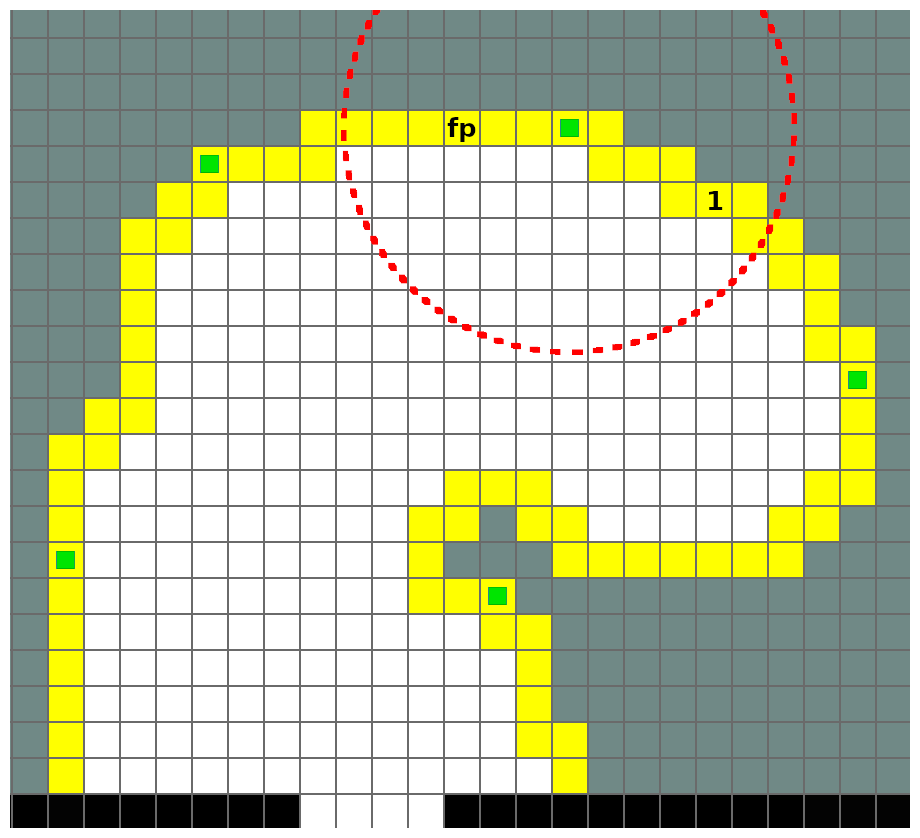
\includegraphics[clip=true, width=0.40\textwidth]{imagenes/ejemploSimpCub/f4.png}}


  \subfloat[$\mli{UF}=\emptyset$ por lo que el algorimo finaliza.]{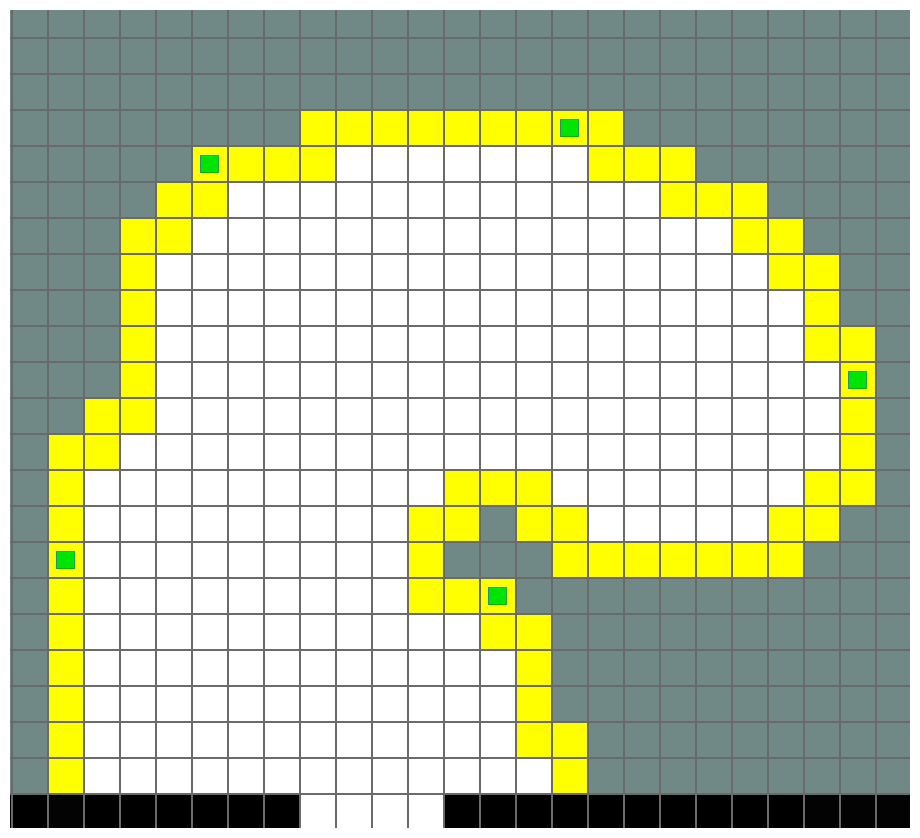
\includegraphics[clip=true, width=0.40\textwidth]{imagenes/ejemploSimpCub/zfinal1.png}}
  % \subfloat[$\mli{UF}=\emptyset$ por lo que el algorimo finaliza.]{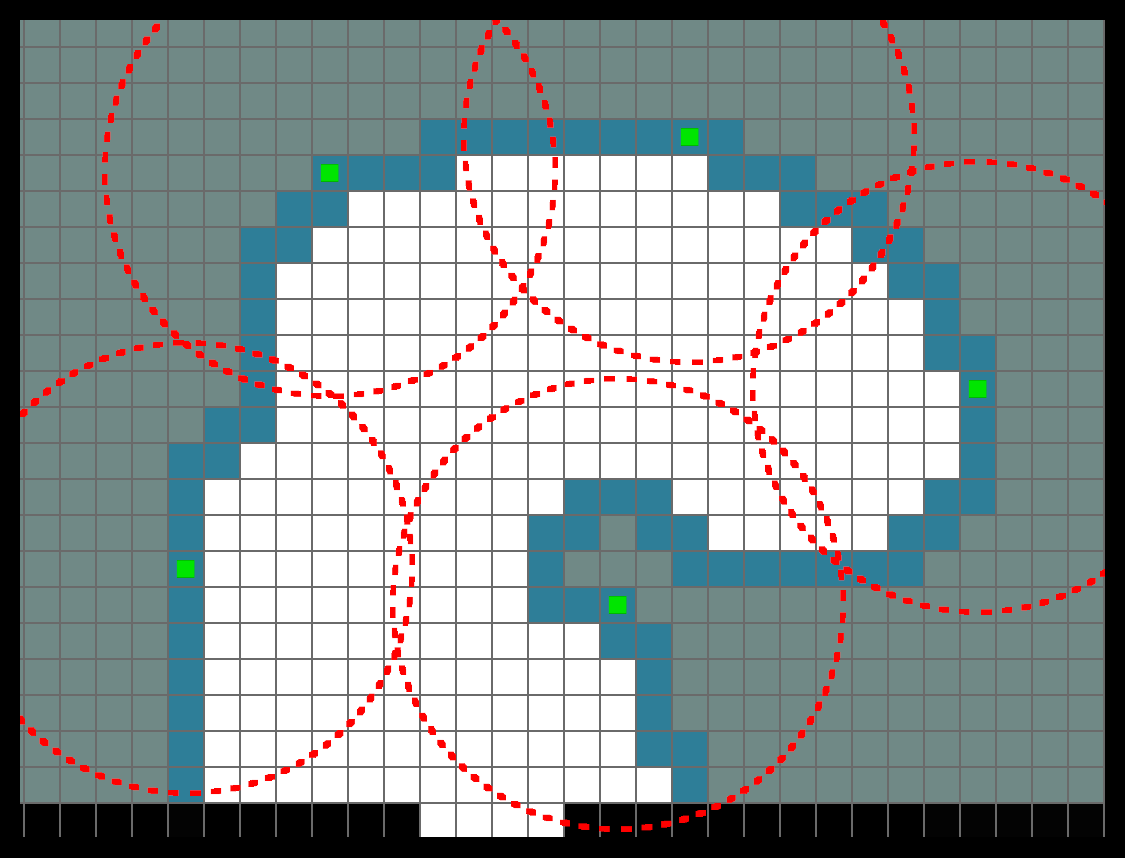
\includegraphics[clip=true, width=0.40\textwidth]{imagenes/ejemploSimpCub/zfinal3.png}}

  \caption[Proceso de simplificacion de fronteras según cubrimiento.]{Proceso
    de simplificacion de fronteras según cubrimiento. Las fronteras de $F_i$ se
    indican con azul si pertenecen a $\mli{UF}$ y con amarillo de lo contrario.
    Con magenta se indican las celdas en $\mli{FP}$ siendo la numeracion su
    orden en la cola y $\mli{fp}$ la ultima desencolada. Las
    circunferencias rojas centradas en $\mli{fp}$ tienen como radio la distancia
    utilizada para obtener los candidatos $\mli{FSC}$ los cuales se indican con
    naranja. Las fronteras significativas se indican con verde, siendo las
    circunferencias rojas de radio $rango=5.6$ (largos de celda) centradas en estas indicadores de su
  cubrimiento.}\label{fig:ejemploFSCubComp}

\end{figure}
